\documentclass[10pt]{IEEEtran}
\usepackage[spanish]{babel}
\usepackage[utf8]{inputenc}
\usepackage{graphicx}
\usepackage{subfigure} 
\usepackage{amsmath}
\usepackage{float}



\title {Operación XOR de manera cruzada en mapas Renyi donde $i =j$, aplicación de pruebas NIST.}

\author{\IEEEauthorblockN{Marcos Daniel Calderón Calderón}\\
\IEEEauthorblockA{Maestría en Ciencias de la Computación\\
Centro de Investigación en Matemáticas (CIMAT)\\
Guanajuato , Gto.\\
marcos.calderon@cimat.mx}}


\begin{document}
\maketitle
\begin{abstract}
En este reporte se explica de manera detallada el funcionamiento de una operación XOR de manera cruzada entre la parte inferior y superior de dos números por mapas caóticos Renyi.
\end{abstract}
\section{Introducción.}

EL mapa caótico Renyi tiene la siguiente forma:

\begin{equation}
f(k)=  \left(  q2^{n-i}k +  \lfloor \frac{k}{2^{j}} \rfloor   \right) \mod{ 2^{n}}
\end{equation}.


Ahora, para facilitar la explicación, supongamos que estamos trabajando con datos de 8 bits. Esto significa que cada número se puede dividir en dos partes de 4 bits, la parte izquierda es la más significativa, la parte derecha es la menos significativa. Supongamos que vamos a trabajar con los siguientes datos:

\begin{equation}
x_{1}=103 \quad    (0110 0111)
\quad \quad 
x_{2}=89 \quad     (0101 1001)
\end{equation}


También, necesitamos un valor auxiliar:
\begin{equation}
a=15  \quad  \quad   (0000 1111)
\end{equation}

El esquema que se manejará es el siguiente:
\begin{figure}[H]
\centering
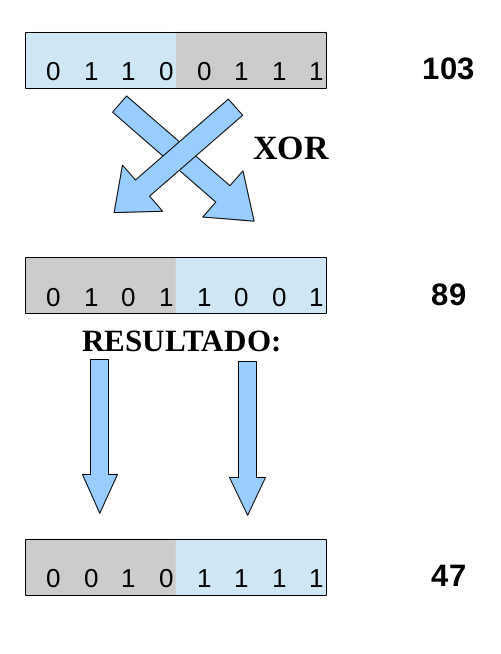
\includegraphics[width=7cm]{es.jpg}
\caption{Esquema de intercambio.}
\label{vovo}
\end{figure}

Un código simplificado (para ocho bits) que hace la operación anterior es el siguiente:
\begin{verbatim}

   char a = 15;
   char temp;
   char temp1;
   char temp2;
   char Xn1;
   char Xn2;
   char Xn3;
   Xn1=103;
   Xn2= 89;
            temp1 = Xn2 & a;
            temp2 = Xn1 >> 4;
            temp = temp1^temp2;
            temp1 = Xn2 >> 4;
            temp2 = Xn1 & a;
            Xn3=(temp1^temp2)<<4;
            Xn3|=temp;
\end{verbatim}


Ahora, para los ejemplos que se muestran aquí se utilizan 32 bits, esto significa que se van a dividir los datos generados por los mapas caóticos en dos partes: cada una de 16 bits. También, en este caso, necesitamos un nuevo valor para a: $(a = 2^{16}-1= 65,535)$



\section{Ejemplo 1.}

\subsection{Procedimiento.}

Para que el mapa sea invertible, es necesario que se cumpla la siguiente condición:

\begin{equation}
0 < i  = j \leq n
\end{equation}

por lo tanto, hemos elegido los siguientes parámetros:



\begin{itemize}
\item Mapa 1: $i = j = 9$.


\item Mapa 2: $i = j = 13$.
\end{itemize}

Ahora, es necesario elegir un valor de $q$ adecuado, en este ejemplo, utilizamos los siguientes:

\begin{itemize}
\item Mapa 1: $q = 13.$
\item Mapa 2: $q = 19.$
\end{itemize}


Ahora, es necesario calcular el parámetro que se forma de la expresión:  
\begin{equation}
\beta = q 2^{n-i}
\end{equation}
con base en lo anterior, se encontraron los siguientes parámetros para el mapa 1 y el mapa 2 respectivamente:

\begin{itemize}
\item $\beta_{1}=109051904$.
\item $\beta_{2}=9961472$.
\end{itemize}



 
También es importante elegir el tipo de dato que se va a utilizar para almacenar los valores generados por los mapas, en este caso se eligió el tipo de dato \textbf{unsigned long} (se utilizó un equipo con arquitectura de 32 bits, donde este tipo de dato tiene un tamaño de 32 bits).

Se generaron 80,000 valores  a la hora de relacionar los valores de los dos mapas con la operación XOR. Como cada valor está formado de 32 bits, se  obtiene un total de $2,560,000$ bits para la aplicación de pruebas NIST.





Se utilizó el siguiente código para la ejecución de las pruebas NIST:

Se ejecutó el siguiente código:

\begin{itemize}
\item \textbf{./assess 2560000}
\item User Prescribed Input File: \textbf{dosRenyisINtercambio1.dat}
\item    Enter 0 if you DO NOT want to apply all of the
         statistical tests to each sequence and 1 if you DO. Enter chice: \textbf{1}
                  
\item  How many bitstreams? \textbf{1}

\item Input File Format:
    [0] ASCII - A sequence of ASCII 0's and 1's
    [1] Binary - Each byte in data file contains 8 bits of data

   Select input mode:  \textbf{1}
\end{itemize}

\subsection{Resultados.}
Los resultados obtenidos son los siguientes:


\begin{table}[H]
\centering
\caption{Primeros 3 datos obtenidos en el ejemplo 1.}
\begin{tabular}[c]{|c|c|c|}
\hline

\multicolumn{3}{|c|}{Primeros tres valores generados con el esquema propuesto.}\\
\hline

\hline

\multicolumn{3}{|c|}{Primer valor generado }\\
\hline
Especificación  & Base 10 & Representación binaria \\
\hline
Valor mapa 1 &  1417674752  & 
0101010010000000  0000000000000000
 \\

\hline
Valor mapa 2 &  189267968  & 0000101101001000  0000000000000000 \\
\hline
Resultado  & 189289600 &  0000101101001000 0101010010000000 \\
\hline
\hline

\multicolumn{3}{|c|}{ Segundo valor generado }\\
\hline
Especificación  & Base 10 & Representación binaria \\
\hline
Valor mapa 1 &  2768896  & 0000000000101010 0100000000000000  \\

\hline
Valor mapa 2 &  23104  & 0000000000000000 0101101001000000 \\
\hline
Resultado  & 1073764970   &  0100000000000000 0101101001101010  \\
\hline
\hline

\multicolumn{3}{|c|}{Tercer valor generado }\\
\hline
Especificación  & Base 10  & Representación binaria \\
\hline
Valor mapa 1 &  5408  &  0000000000000000 0001010100100000  \\

\hline
Valor mapa 2 &  2516582402  &  1001011000000000 0000000000000010  \\
\hline
Resultado  &  2199912450  &  1000001100100000 0000000000000010 \\

\hline
\hline
\end{tabular}
\end{table}

 

\begin{table}[H]
\caption{Resultados de las pruebas de aleatoriedad NIST a los datos dosRenyisIntercambio1.dat .}
\label{sample-table}
\vskip 0.15in
\begin{center}
\begin{small}
\begin{sc}
\begin{tabular}{lccr}
\hline

Prueba Aplicada &  P-Valor & Exito? \\
\hline

Aproximate Entropy    &  0.128865 & $\surd$ \\

Block Frecuency  &  0.404371 &  $\surd$  \\

Cumulative Sums    &   F: 0.503743, R: 0.542327  & $\surd$ \\

FFT    &   0.679644  &   $\surd$      \\

Frecuency     &  0.963111 &  $\surd$   \\

Linear Complexity      &  0.778769  & $\surd$ \\

Longest Run      & 0.455532 &    $\surd$      \\

Non Overlapping Template      &  146 de 148    &     $\surd$          \\

Overlapping Template      &  0.089385  &        $\surd$       \\

Random Excursions      &  7 de 8  &    $\surd$      \\

Random Excursions Variant &  18 de 18 &     $\surd$    \\

Rank &   0.699856  &      $\surd$      \\

Runs &   0.950166 &     $\surd$        \\

Serial &     2 de 2    &     $\surd$        \\

Universal &      0.086113  &   $\surd$            \\

\hline



\end{tabular}
\end{sc}
\end{small}
\end{center}
\vskip -0.1in
\end{table}


 
\section{Ejemplo 2.}

\subsection{Procedimiento.}
Para el ejemplo 2, se eligieron los siguientes parámetros:

\begin{itemize}
\item Mapa 1: $i = j = 5$.


\item Mapa 2: $i = j = 14$.
\end{itemize}

Ahora, es necesario elegir un valor de $q$ adecuado, en este ejemplo, utilizamos los siguientes:

\begin{itemize}
\item Mapa 1: $q = 29.$
\item Mapa 2: $q = 31.$
\end{itemize}


Ahora, es necesario calcular el parámetro que se forma de la expresión:  
\begin{equation}
\beta = q 2^{n-i}
\end{equation}
con base en lo anterior, se encontraron los siguientes parámetros para el mapa 1 y el mapa 2 respectivamente:

\begin{itemize}
\item $\beta_{1}=3892314112$.
\item $\beta_{2}=8126464$.
\end{itemize}







\subsection{Resultados.}


Se utilizó el siguiente código para la ejecución de las pruebas NIST:


\begin{itemize}
\item \textbf{./assess 2560000}
\item User Prescribed Input File: \textbf{dosRenyisIntercambio2.dat}
\item    Enter 0 if you DO NOT want to apply all of the
         statistical tests to each sequence and 1 if you DO. Enter chice: \textbf{1}
                  
\item  How many bitstreams? \textbf{1}

\item Input File Format:
    [0] ASCII - A sequence of ASCII 0's and 1's
    [1] Binary - Each byte in data file contains 8 bits of data

   Select input mode:  \textbf{1}
\end{itemize}

Los resultados obtenidos son los siguientes:


\begin{table}[H]
\centering
\caption{Primeros 3 datos obtenidos en el ejemplo 2.}
\begin{tabular}[c]{|c|c|c|}
\hline

\multicolumn{3}{|c|}{Primeros tres valores generados con el esquema propuesto.}\\
\hline

\hline

\multicolumn{3}{|c|}{Primer valor generado }\\
\hline
Especificación  & Base 10 & Representación binaria \\
\hline
Valor mapa 1 & 3355443200   &  1100 1000 0000 0000 0000 0000 0000 0000\\

\hline
Valor mapa 2 &  154402816  & 0000 1001 0011 0100 0000 0000 0000 0000 \\
\hline
Resultado  &  154454016  &  0000 1001 0011 0100 1100 1000 0000 0000\\
\hline
\hline

\multicolumn{3}{|c|}{ Segundo valor generado }\\
\hline
Especificación  & Base 10 & Representación binaria \\
\hline
Valor mapa 1 & 104857600  & 0000 0110 0100 0000 0000 0000 0000 0000  \\

\hline
Valor mapa 2 &   9424   & 0000 0000 0000 0000 0010 0100 1101 0000\\
\hline
Resultado  & 8848    & 0000 0000 0000 0000 0010 0010 1001 0000  \\
\hline
\hline

\multicolumn{3}{|c|}{Tercer valor generado }\\
\hline
Especificación  & Base 10  & Representación binaria \\
\hline
Valor mapa 1 &  3276800  & 0000 0000 0011 0010 0000 0000 0000 0000  \\

\hline
Valor mapa 2 &  3569352704   &  1101 0100 1100 0000 0000 0000 0000 0000  \\
\hline
Resultado  &  3569352754   & 1101 0100 1100 0000 0000 0000 0011 0010 \\
\hline
\hline

\hline
\hline
\end{tabular}
\end{table}

 
 

\begin{table}[H]
\caption{Resultados de las pruebas de aleatoriedad NIST a los datos dosRenyisIntercambio2.dat .}
\label{sample-table}
\vskip 0.15in
\begin{center}
\begin{small}
\begin{sc}
\begin{tabular}{lccr}
\hline

Prueba Aplicada &  P-Valor & Exito? \\
\hline

Aproximate Entropy    &   0.847752 & $\surd$ \\

Block Frecuency  & 0.330180  &  $\surd$  \\

Cumulative Sums    &   F:0.170864, R: 0.109874  & $\surd$ \\

FFT    &   0.774289 &   $\surd$      \\

Frecuency     &  0.167972 &  $\surd$   \\

Linear Complexity      & 0.712980 & $\surd$ \\

Longest Run      &  0.516759 &    $\surd$      \\

Non Overlapping Template      & 146 de 148    &     $\surd$          \\

Overlapping Template      &  0.563560  &        $\surd$       \\

Random Excursions      & 8 de 8  &    $\surd$      \\

Random Excursions Variant & 18 de 18 &     $\surd$    \\

Rank &   0.648994  &      $\surd$      \\

Runs &   0.618793 &     $\surd$        \\

Serial &     2 de 2    &     $\surd$        \\

Universal &       0.227311&   $\surd$            \\

\hline



\end{tabular}
\end{sc}
\end{small}
\end{center}
\vskip -0.1in
\end{table}



\section{Conclusiones.}

Se obtuvieron resultados satisfactorios a la hora de aplicar las pruebas NIST a los datos generados por el esquema ropuesto. En este caso, se supuso que $i = j$. 

Normalmente ocurre que si se obtienen trayectorias aceptables de los mapas utilizados al aplicar el esquema que se menciona en este documento, se obtendrán valores que aprobarán las pruebas NIST.

\onecolumn
\section{Anexos.}

\subsection{Codigo Ejemplo 1.}
\begin{verbatim}
#include <stdio.h>
#include <stdlib.h>
#include <math.h>

#define RENYI_MAP(var, parametro, j) ((var)*(parametro)+((var)>>(j)))
#define ITtotales 80000 /*Iteraciones totales para NIST.*/

/*
 File:   main.c
 Author: daniel
En este programa, hacemoxs un esquema cruzado para la generacion de numeros
aleatorios.
*/

unsigned long calcular_parametro(unsigned long q, unsigned int n, unsigned int i){    
    unsigned long potencia =1;
    unsigned int j;
    /*Calculo de la potencia (calculamos 2(a la)( n-i) ): */
    for(j =0; j<(n-i); j++){
        potencia*=2;
    }

    /*Ahora, lo que hacemos es la operacion q*2(a la )(n-i): */
    unsigned long parametro = q*(potencia);
    printf("  EL parametro es: %lu \n \n \n",parametro);
    return parametro;
}

int main(){
 
   
  /*En este primer ejemplo, se hace la prueba para i = j en cada uno de 
   los dos mapas.*/
   unsigned long Xtotal[ITtotales]; 
   FILE *  archivobin; 
   unsigned long Xn1 = 13;
   unsigned long Xn2 = 19;
   unsigned int n = 32;

   /*Valores de i, j y q para el mapa 1.*/
   unsigned int i1=9; 
   unsigned int j1=9; 
   unsigned long q1=13;
   /*Valores de i, j y q para el mapa 2.*/
   unsigned int i2=13; 
   unsigned int j2=13; 
   unsigned long q2=19;
 
   /*Calculo de los parametros para cada mapa: 1 y 2 respectivamente.*/
   unsigned long param1 =calcular_parametro(q1, n, i1);
   unsigned long param2 =calcular_parametro(q2, n, i2);
 
   unsigned int iteraciones=0;
   unsigned int IT = 80000;

  /* Apertura del fichero de destino, para escritura en binario.*/
   archivobin = fopen ("dosRenyisIntercambio1.dat", "wb");
   if (archivobin==NULL)
   {
   perror("No se puede abrir dosRenyisIntercambio1.dat");
   return -1;
   }
   
   printf("\n\n\n Operacion XOR en dos Renyis \n EL tamanio
    de unsigned long en maquina de 32 bits es:  %d", sizeof(long));


  /*Sea a el valor de 2^16 -1 (el maximo valor en 16 bits de 32.)*/
   unsigned long a = 65535;
   /*Declaramos valores temporales.*/
   unsigned long temp;
   unsigned long temp1;
   unsigned long temp2;
   unsigned long Xn3;

   while (iteraciones < IT) {

           /*Primero, creamos los valores por medio del mapa renyi.*/
            Xn1= RENYI_MAP(Xn1,param1,j1);
            Xn2= RENYI_MAP(Xn2,param2,j2);

            /*obtenemos la parte derecha del valor de Xn2.*/
            temp1 = Xn2 & a;
            /*Obtenemos la parte izquierda del valor de Xn1.*/
            temp2 = Xn1 >> 16;
            /*Hacemos la combinacion.*/
            temp = temp1^temp2;

            /*Obtenemos la parte izquierda del valor de x2.*/
            temp1 = Xn2 >> 16;
            /*Obtenemos la parte derecha del valor de x1.*/
            temp2 = Xn1 & a;
            
            /*Ahora, formamos el nuevo valor para x3.*/
            Xn3=(temp1^temp2)<<16;
            Xn3|=temp;


            Xtotal[iteraciones++] = Xn3;
 
 

   } 
 

   /*Escribimos la informacion.*/
   fwrite(Xtotal,4,80000,archivobin); 

   if(!fclose(archivobin)){
      printf( "\nArchivo binario intercambio 1 cerrado\n" );
   }
   else{
      printf( "\nError: Archivo binario intercambio 1 no cerrado \n" );
      return 1;
   }  

  

return 0;
}
\end{verbatim}

\subsection{Codigo Ejemplo 2.}
\begin{verbatim}
#include <stdio.h>
#include <stdlib.h>
#include <math.h>

#define RENYI_MAP(var, parametro, j) ((var)*(parametro)+((var)>>(j)))
#define ITtotales 80000 /*Iteraciones totales para NIST.*/

/*
 File:   main.c
 Author: daniel
En este programa, hacemoxs un esquema cruzado para la generacion de numeros
aleatorios.
*/

unsigned long calcular_parametro(unsigned long q, unsigned int n, unsigned int i){    
    unsigned long potencia =1;
    unsigned int j;
    /*Calculo de la potencia (calculamos 2(a la)( n-i) ): */
    for(j =0; j<(n-i); j++){
        potencia*=2;
    }

    /*Ahora, lo que hacemos es la operacion q*2(a la )(n-i): */
    unsigned long parametro = q*(potencia);
    printf("  EL parametro es: %lu \n \n \n",parametro);
    return parametro;
}

int main(){
 
   
   /*Declaramos los arreglos que vamos a utilizar para guardar esto. EL tipo de dato será
   unsigned int, cuyo tamaño es de 34 bits (arquitectura de 64 bits).*/
   unsigned long Xtotal[ITtotales]; 
   FILE *  archivobin; 
   unsigned long Xn1 = 13;
   unsigned long Xn2 = 19;
   unsigned int n = 32;

   /*Valores de i, j y q para el mapa 1.*/
   unsigned int i1=5; 
   unsigned int j1=5; 
   unsigned long q1=29;
   /*Valores de i, j y q para el mapa 2.*/
   unsigned int i2=14; 
   unsigned int j2=14; 
   unsigned long q2=31;
 
   /*Calculo de los parametros para cada mapa: 1 y 2 respectivamente.*/
   unsigned long param1 =calcular_parametro(q1, n, i1);
   unsigned long param2 =calcular_parametro(q2, n, i2);
 
   unsigned int iteraciones=0;
   unsigned int IT = 80000;

  /* Apertura del fichero de destino, para escritura en binario.*/
   archivobin = fopen ("dosRenyisIntercambio2.dat", "wb");
   if (archivobin==NULL)
   {
   perror("No se puede abrir dosRenyisIntercambio2.dat");
   return -1;
   }
   
   printf("\n\n\n Operacion XOR en dos Renyis \n EL tamanio 
   de unsigned long en maquina de 32 bits es:  %d", sizeof(long));

  /*Sea a el valor de 2^16 -1 (el maximo valor en 16 bits de 32.)*/
   unsigned long a = 65535;
   /*Declaramos valores temporales.*/
   unsigned long temp;
   unsigned long temp1;
   unsigned long temp2;
   unsigned long Xn3;


   while (iteraciones < IT) {

            /*Primero, creamos los valores por medio del mapa renyi.*/
            Xn1= RENYI_MAP(Xn1,param1,j1);
            Xn2= RENYI_MAP(Xn2,param2,j2);

            /*obtenemos la parte derecha del valor de Xn2.*/
            temp1 = Xn2 & a;
            /*Obtenemos la parte izquierda del valor de Xn1.*/
            temp2 = Xn1 >> 16;
            /*Hacemos la combinacion.*/
            temp = temp1^temp2;

            /*Obtenemos la parte izquierda del valor de x2.*/
            temp1 = Xn2 >> 16;
            /*Obtenemos la parte derecha del valor de x1.*/
            temp2 = Xn1 & a;
            
            /*Ahora, formamos el nuevo valor para x3.*/
            Xn3=(temp1^temp2)<<16;
            Xn3|=temp;


            Xtotal[iteraciones++] = Xn3;
             
         
   } 
 

   /*Escribimos la informacion.*/
   fwrite(Xtotal,4,80000,archivobin); 

   if(!fclose(archivobin)){
      printf( "\nArchivo binario intercambio 2 cerrado\n" );
   }
   else{
      printf( "\nError: Archivo binario  intercambio 2 no cerrado \n" );
      return 1;
   }  

  

return 0;
}
\end{verbatim}

\end{document}


